\documentclass[11pt]{book}
\usepackage{palatino}
\usepackage{amsfonts,amsmath,amssymb}

% Packages for Figures:
% Without conversion of eps to pdf:
\usepackage{graphicx}
% With conversion of eps to pdf,
% which depends on platform.
%\ifx\pdftexversion\undefined
%    \usepackage[dvips]{graphicx}
%\else
%    \usepackage[pdftex]{graphicx}
%    \usepackage{epstopdf}
%    \epstopdfsetup{suffix=}
%\fi

% Packages for displaying code:
\usepackage{listings}
\usepackage{textcomp}
\usepackage{color}

% Color settings used in the code below:
\definecolor{dkgreen}{rgb}{0,0.6,0}
\definecolor{gray}{rgb}{0.5,0.5,0.5}
\definecolor{mauve}{rgb}{0.58,0,0.82}

% Settings for the formatting of the code on display:
\lstset{frame=tb,
  language=R,
  aboveskip=3mm,
  belowskip=3mm,
  showstringspaces=false,
  columns=flexible,
  basicstyle={\small\ttfamily},
  numbers=none,
  numberstyle=\tiny\color{gray},
  keywordstyle=\color{blue},
  commentstyle=\color{dkgreen},
  stringstyle=\color{mauve},
  breaklines=true,
  breakatwhitespace=true,
  tabsize=3
}

% Package for displaying inline verbatim commands in footnotes.
\usepackage{fancyvrb}


\begin{document}

%%%%%%%%%%%%%%%%%%%%%%%%%%%%%%%%%%%%%%%%
% Problem Set 4
%%%%%%%%%%%%%%%%%%%%%%%%%%%%%%%%%%%%%%%%

\pagestyle{empty}
{\noindent\bf Spring 2021 \hfill Firstname M.~Lastname}
\vskip 16pt
\centerline{\bf University of Central Florida}
\centerline{\bf College of Business}
\vskip 16pt
\centerline{\bf QMB 6911}
\centerline{\bf Capstone Project in Business Analytics}
\vskip 10pt
\centerline{\bf Solutions:  Problem Set \#5}
\vskip 32pt
\noindent

\section{Introduction}

This note summarizes the findings in the script
\texttt{Tractor\_Data\_Vis.R},
which analyzes the prices of used tractors,
the dependent variable in the \texttt{TRACTOR7.csv} dataset.
The output includes several plots of the
dependent variable against the explanatory variables.

The primary goal is to determine the relative value of John Deere tractors compared to others.
A secondary consideration is to determine the time of year in which to
sell a tractor.

\vfill
\pagebreak
\section{Histogram and Density of Log. Tractor Prices}


\subsection{All Tractors Together}

Start with the log of sale prices because that
seemed more promising, given that prices were highly skewed.

\begin{lstlisting}[language=R]
hist(tractor_sales[, 'log_saleprice'],
     main = 'Histogram and Density of Log. Tractor Prices',
     xlab = 'Price', col = 'red',
     probability = TRUE)
rug(tractor_sales[, 'log_saleprice'])
lines(density(tractor_sales[, 'log_saleprice']),
      col = 'blue', lwd = 3)
\end{lstlisting}


Figure \ref{fig:hist_dens_log_price} is
a histogram of the logarithm of tractor prices,
along with a rug plot and a kernel density estimate,
generated by the code block above.
%
\begin{figure}[h!]
  \centering
  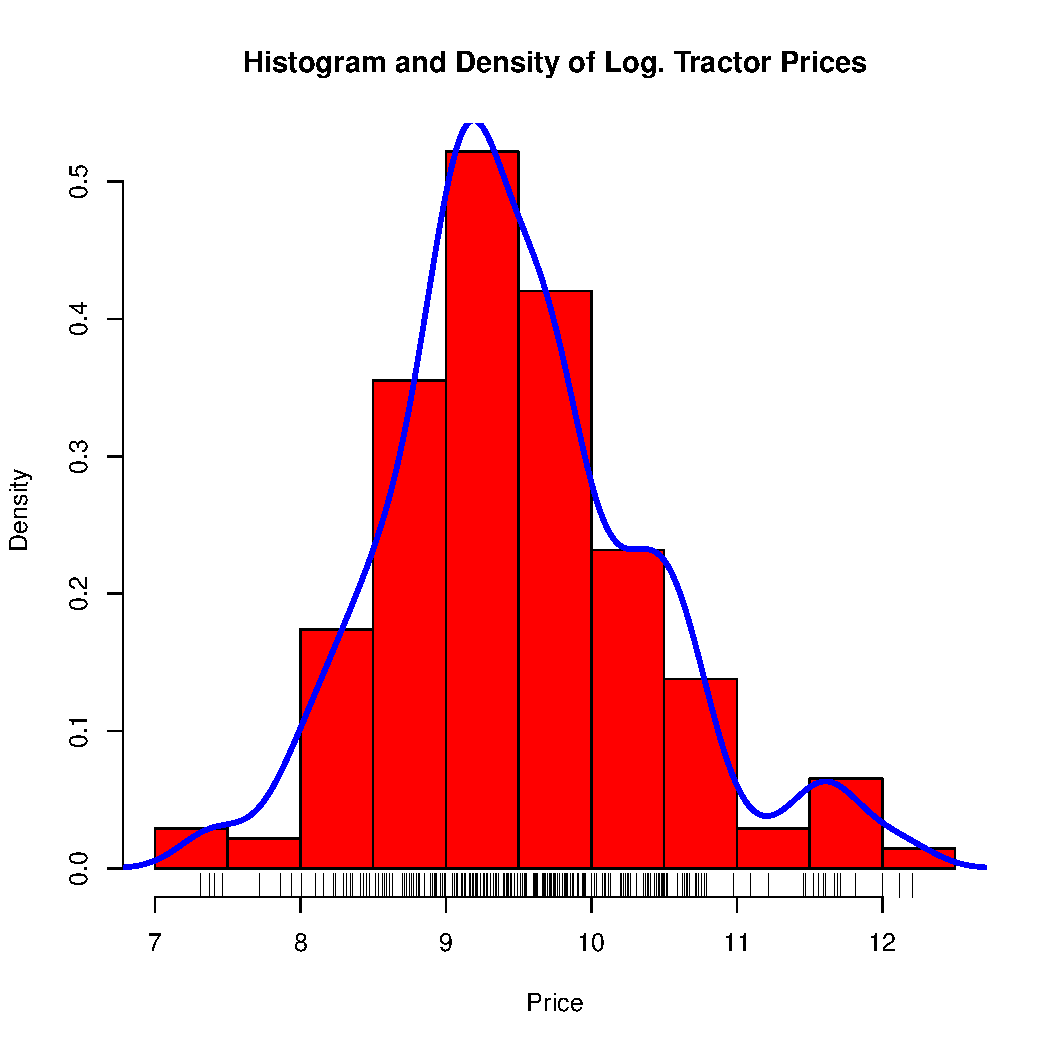
\includegraphics[scale = 0.5, keepaspectratio=true]{../Figures/hist_dens_log_price}
  \caption{Relative Histogram of Tractor Prices} \label{fig:hist_dens_log_price}
\end{figure}
%
After taking logs, we can see that the distribution is
approximately symmetric, with some bunching in the
upper tail.

\pagebreak
\subsection{Comparison By Make}

Now we investigate the value of John Deere tractors
compared to other brands.
Figure \ref{fig:dens_by_brand} shows the
kernel density estimate of the sale prices of John Deere tractors
in green and that of the other brands in red.
%
The distribution of sale prices of John Deere tractors has several modes and is skewed to the right,
with the highest mode lower than that for other brands.


\begin{lstlisting}[language=R]
library(sm)
sm.density.compare(tractor_sales[, 'log_saleprice'],
                   tractor_sales[, 'johndeere'],
                   xlab = "Log. of Sale Price",
                   lwd = 3,
                   col = c('red','green'))
title(main = "Log. of Sale Price by Brand")
legend('topright', c('Other', 'John Deere'),
       fill = c('red','green'),
       cex = 0.75)
\end{lstlisting}


\begin{figure}[h!]
  \centering
  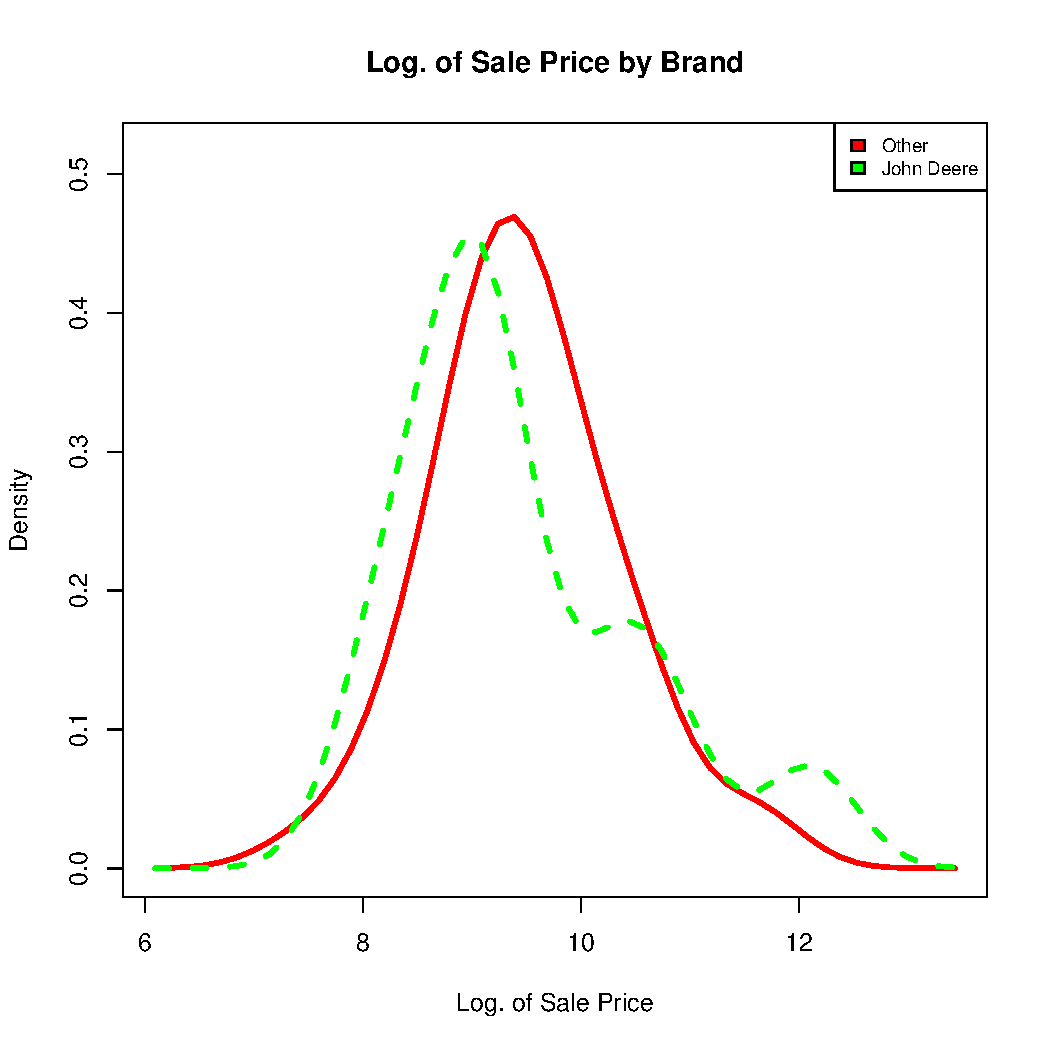
\includegraphics[scale = 0.5, keepaspectratio=true]{../Figures/dens_by_brand}
  \caption{Densities of Log. Tractor Prices by Brand} \label{fig:dens_by_brand}
\end{figure}


\pagebreak
\subsection{Comparison By Season of Sale}

Figure \ref{fig:dens_by_season} shows
the densities of the logarithm of sales price,
separated by the season of the year in which they were sold.
The figure was generated by the following code.
%
\vfill

\begin{lstlisting}[language=R]
plot(density(tractor_sales[tractor_sales[, 'fall'] == 1, 'log_saleprice']),
     col = 'orange',
     lwd = 3,
     xlim = c(min(tractor_sales[, 'log_saleprice']),
              max(tractor_sales[, 'log_saleprice'])),
     main = 'Log. of Sale Price by Season of Sale')
# Plot the rest.
lines(density(tractor_sales[tractor_sales[, 'spring'] == 1, 'log_saleprice']),
     col = 'green',
     lwd = 3)
lines(density(tractor_sales[tractor_sales[, 'summer'] == 1, 'log_saleprice']),
      col = 'yellow',
      lwd = 3)
lines(density(tractor_sales[tractor_sales[, 'winter'] == 1, 'log_saleprice']),
      col = 'blue',
      lwd = 3)
legend('topright',
       c('Spring', 'Summer', 'Fall', 'Winter'),
       fill = c('green', 'yellow', 'orange', 'blue'),
       cex = 0.65)
\end{lstlisting}

\pagebreak
We see that the distribution of sales is similar
during summer and fall (yellow and orange, respectively)
with some bunching in the upper tail.
We also see more variance in the sale price in winter,
shown in blue.
In the spring, shown in green, the mode of the distribution
is higher.

\begin{figure}[h!]
  \centering
  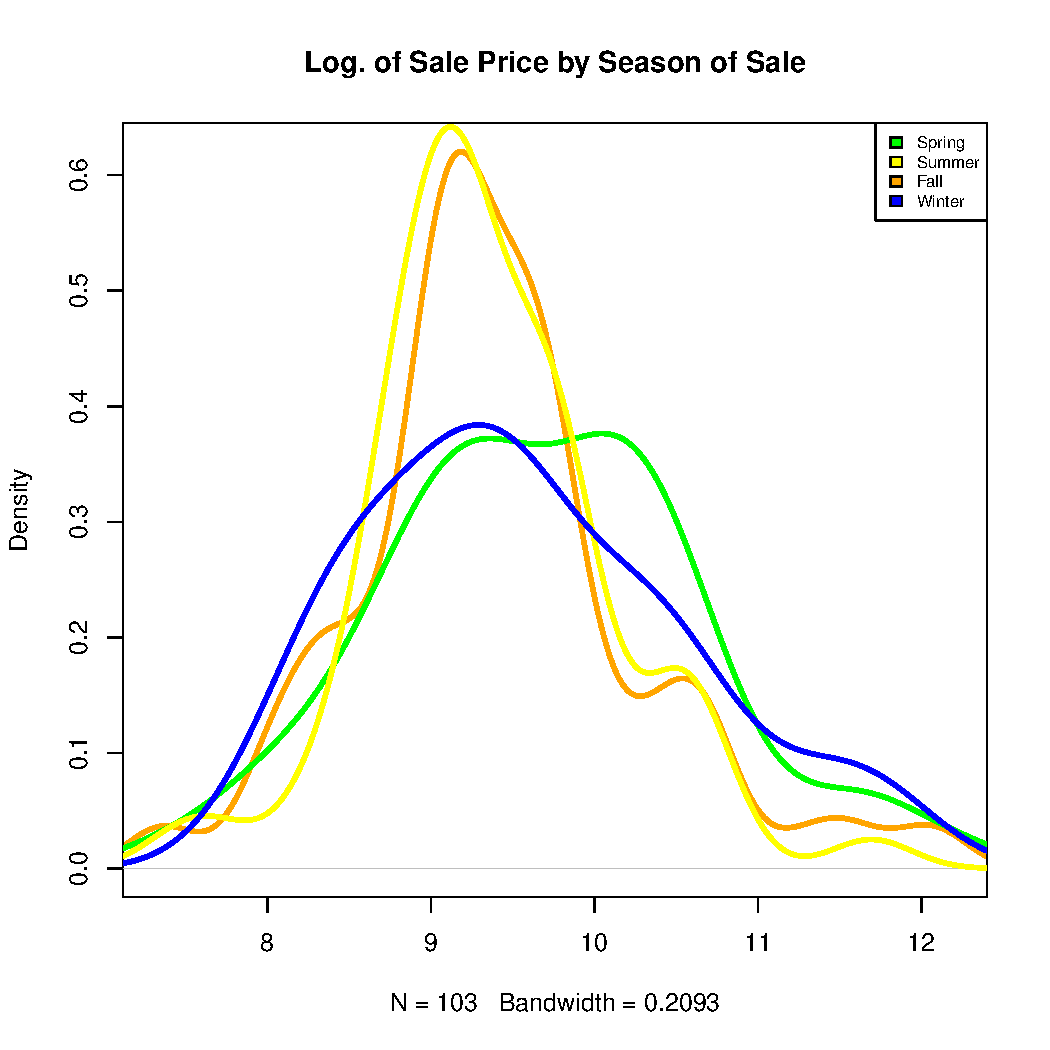
\includegraphics[scale = 0.5, keepaspectratio=true]{../Figures/dens_by_season}
  \caption{Relative Histogram of Tractor Prices} \label{fig:dens_by_season}
\end{figure}


\pagebreak
\section{Sales Volume By Brand and Season of Sale}

Figure \ref{fig:brand_and_season_sales}
shows a spinogram of the number of sales
by brand and the time of year the tractor is sold.
It is generated by the following code.

\begin{lstlisting}[language=R]
# Create a table and plot it in a spinogram.
counts <- table(tractor_sales[, 'season'],
                tractor_sales[, 'JD'])

# Plot the spinogram.
spine(counts,
      main = "Spinogram of Sales by Brand and Season")
\end{lstlisting}

The code block first tabulates the number of sales by
season of sale and whether or not the brand is John Deere.
These counts are shown in Table \ref{tab:brand_and_season_sales}.

% latex table generated in R 4.1.1 by xtable 1.8-4 package
% Tue Feb 15 16:36:40 2022
\begin{table}[ht]
\centering
\begin{tabular}{rrr}
  \hline
 & John Deere & Other \\ 
  \hline
Fall & 14 & 89 \\ 
  Spring & 9 & 53 \\ 
  Summer & 6 & 58 \\ 
  Winter & 10 & 37 \\ 
   \hline
\end{tabular}
\caption{Sales Volume by Brand and Season} 
\label{tab:brand_and_season_sales}
\end{table}


\pagebreak
It appears that sales of John Deere tractors are fairly evenly
distributed throughout the year,
with more sales of John Deere tractors in the winter months
and a fewer sales in the summer.


\begin{figure}[h!]
  \centering
  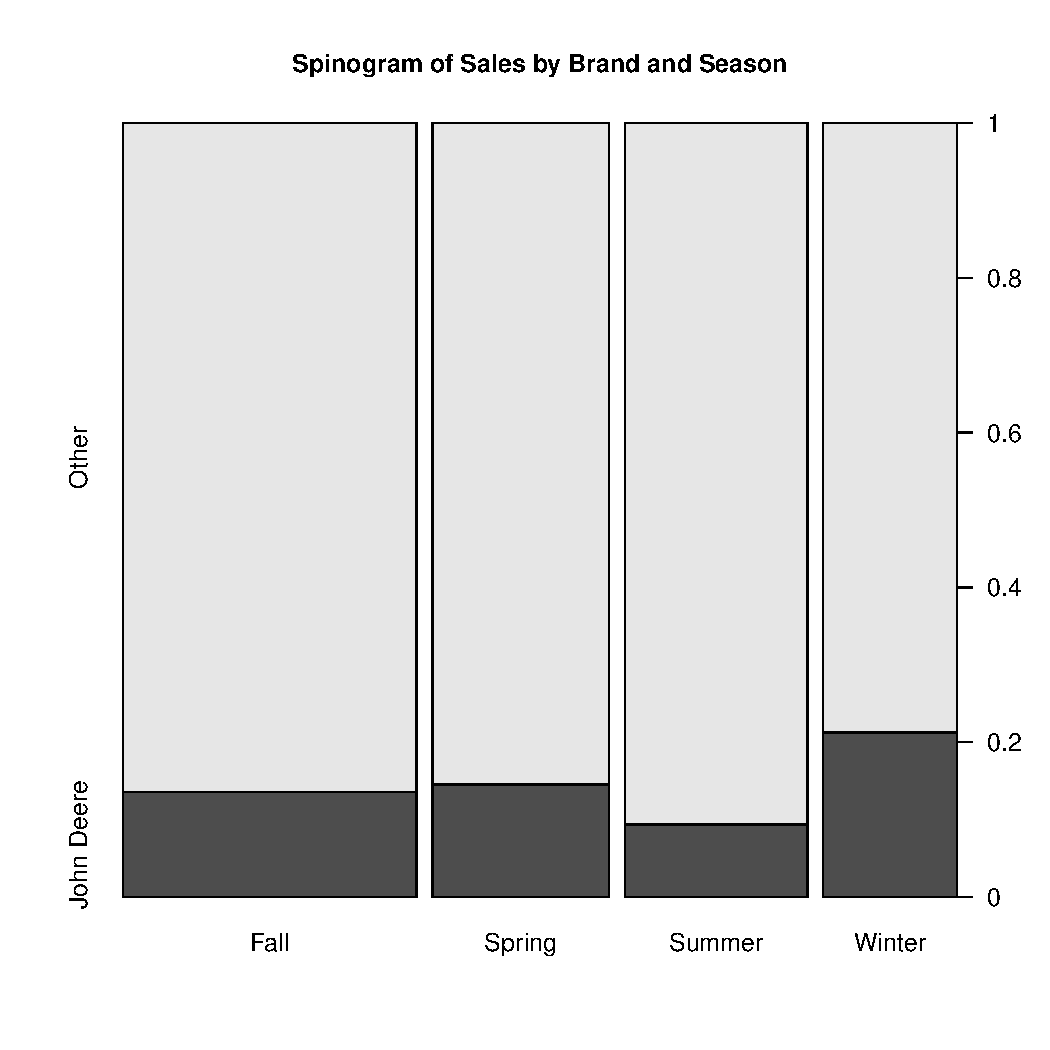
\includegraphics[scale = 0.5, keepaspectratio=true]{../Figures/brand_and_season_sales}
  \caption{Sales Volume of Tractor Prices by Brand and Season of Sale} \label{fig:brand_and_season_sales}
\end{figure}




\pagebreak
\section{Scatterplot Matrix of Numeric Variables}

Figure \ref{fig:scatter_matrix}
shows a scatterplot of the numeric variables in the dataset,
which include
the age in years, the number of engine hours of use,
the number of horsepower produced by the engine,
and the logarithm of the tractor prices.
The \texttt{gclus} package was used to cluster the
correlation matrix to color code by strength of correlation.
The correlation matrix is shown in Table \ref{tab:correlation}.

% latex table generated in R 4.1.1 by xtable 1.8-4 package
% Thu Feb 17 20:55:06 2022
\begin{table}[ht]
\centering
\begin{tabular}{rrrrr}
  \hline
 & Log. of Price & Horsepower & Age & Engine Hours \\ 
  \hline
Log. of Price & 1.000 & 0.649 & -0.441 & -0.046 \\ 
  Horsepower & 0.649 & 1.000 & 0.039 & 0.378 \\ 
  Age & -0.441 & 0.039 & 1.000 & 0.559 \\ 
  Engine Hours & -0.046 & 0.378 & 0.559 & 1.000 \\ 
   \hline
\end{tabular}
\caption{Correlation Matrix of Numeric Variables} 
\label{tab:correlation}
\end{table}


The correlation matrix amd the scatterplot matrix
were generated by the following code.

\begin{lstlisting}[language=R]
# Create a covariance matrix and determine
# parameters for scattergraph matrix.
mydata <- tractor_sales[c(13, 2, 3, 4)]
mydata.corr <- abs(cor(mydata))
mycolors <- dmat.color(mydata.corr)
# Order by magnitude of correlation.
myorder <- order.single(mydata.corr)

# Plot the scatterplot matrix.
cpairs(mydata,
       myorder,
       panel.colors = mycolors,
       gap = 0.5,
       main = c('Scatterplot Matrix Colored by Correlation')
)
\end{lstlisting}


\pagebreak
Horsepower and the logarithm of sale price have strong positive correlation, which is shown in red,
suggesting that tractors with more horsepower are more valuable.
Age and engine hours are also highly correlated
as older tractors have likely been used for more hours.
We also see a modest negative correlation between prices and age,
which makes sense since newer tractors may have new features and may be more reliable.
There appears to be little relation between the
age of a tractor and the horsepower produced by the engine.

\begin{figure}[h!]
  \centering
  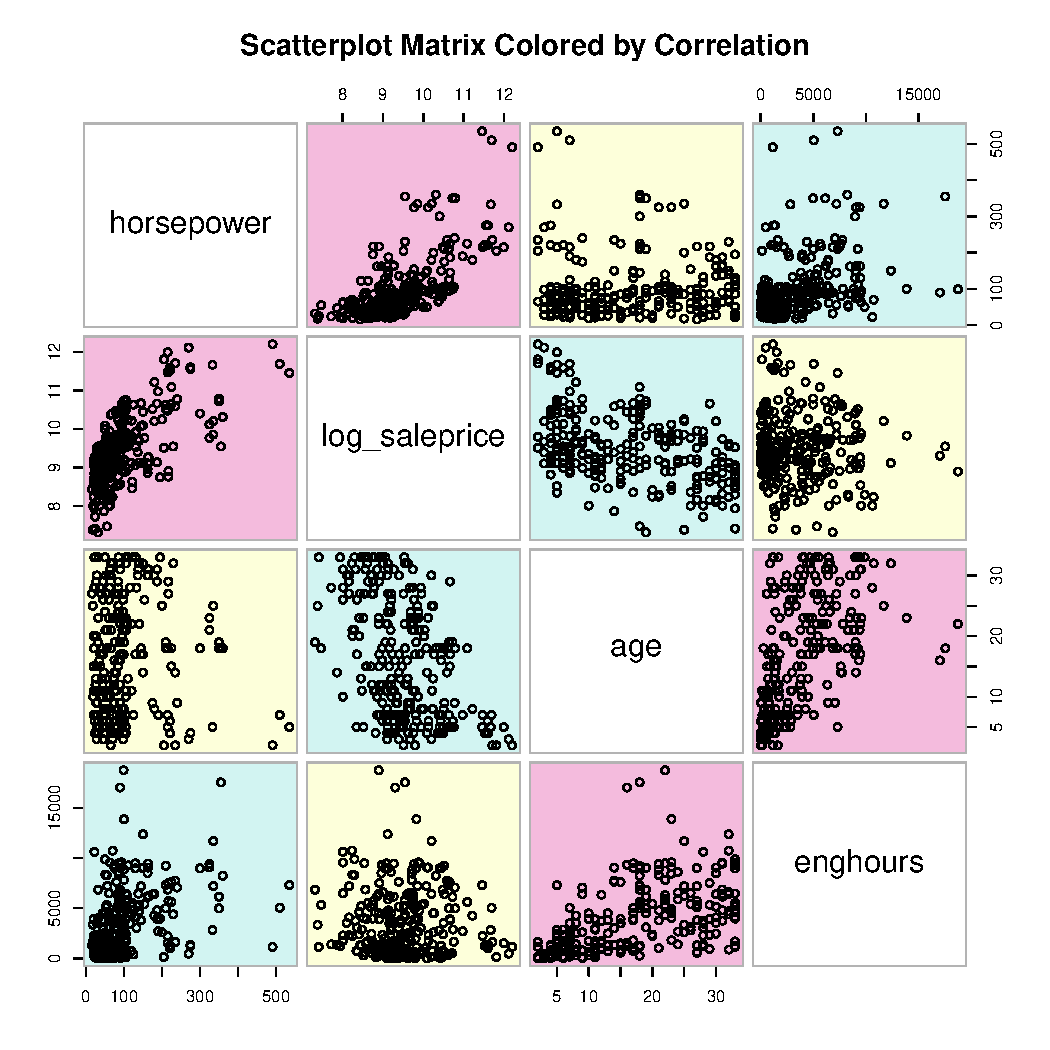
\includegraphics[scale = 0.5, keepaspectratio=true]{../Figures/scatter_matrix}
  \caption{Scatterplot Matrix Colored by Strength of Correlation} \label{fig:scatter_matrix}
\end{figure}



\pagebreak
\section{Relationship between Prices, Horsepower and Age}


Figure \ref{fig:bubble_plot}
shows a bubble plot,
which is a form of scatterplot in which the size of the dots (the ``bubbles'')
represent another variable.
This analysis is based on the above investigation
of the numeric variables in the dataset,
which include
the age in years, the number of engine hours of use,
the number of horsepower produced by the engine,
and the logarithm of the tractor prices.
The logarithm of the tractor prices are shown in the vertical axis,
the age of the tractor is on the horizontal axis,
and the area of each bubble is proportional
to the horsepower of the tractor's engine.
The bubbleplot is
generated by the following code.

\vfill

\begin{lstlisting}[language=R]
# Calculate the radius of the bubbles
# so that the area represents horsepowwer.
r <- sqrt(tractor_sales[, 'horsepower']/pi)

# Plot the bubble plot.
fig_file_name <- 'bubble_plot.pdf'
out_file_name <- sprintf('%s/%s', fig_dir, fig_file_name)
pdf(out_file_name)
symbols(tractor_sales[, 'age'],
        tractor_sales[, 'log_saleprice'],
        r,
        inches=0.30, fg="white", bg="lightblue",
        main = "Bubble Plot with point size proportional to horsepower",
        ylab = "Log. of Sale Price",
        xlab = "Age of Tractor (years)")
\end{lstlisting}


\pagebreak

There appears to be a negative relationship between
the age of a tractor and the sale price.
Also, many of the largest bubbles are concentrated at the higher end of
the price range at each age level.
These findings confirm the results found above in the scatterplots
and covariance matrix.
Together these results indicate that these variables should be included
in some form within a regression model.

\begin{figure}[h!]
  \centering
  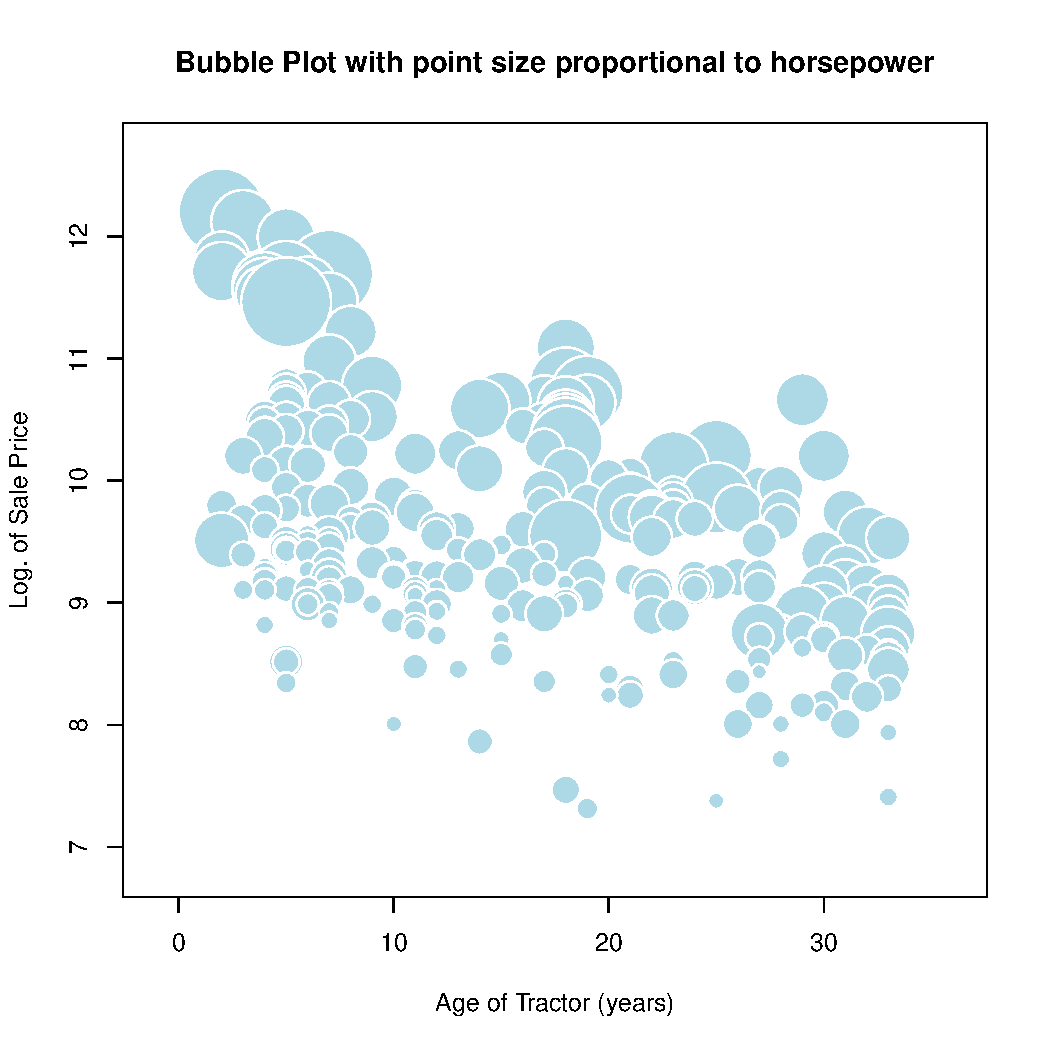
\includegraphics[scale = 0.5, keepaspectratio=true]{../Figures/bubble_plot}
  \caption{Bubble Plot with Point Size Proportional to Horsepower} \label{fig:bubble_plot}
\end{figure}




%%%%%%%%%%%%%%%%%%%%%%%%%%%%%%%%%%%%%%%%
\end{document}
%%%%%%%%%%%%%%%%%%%%%%%%%%%%%%%%%%%%%%%%
